\documentclass{article}
\usepackage[T1]{fontenc}
\usepackage{amsmath}
\usepackage{graphicx}
\graphicspath{{./Documents/}{./figure/}}
\usepackage{multicol}
\begin{document}
\begin{enumerate}
	\item The objective function $Z = ax+by$ of an LLP has maximum value 42 at (4,6) and minimum value 19 at (3,2).Which of the following is true?
		
  		\begin{enumerate}
				\item $a=9,b=1$
		        	\item $a=5,b=2$
				\item $a= 3,b=5$
				\item $a=5,b=3$
			
		\end{enumerate}
		
	\item The corner point of the feasible region of a linear programming problem are (0,4),(8,0)and($\frac{20}{3}$,$\frac{4}{3}$).if $ Z=30x+24y $ is the objective fnction, then ( maximum value of Z-minimum value of Z) is equal to 
		
		\begin{enumerate}
				\item 40
				\item 96
				\item 120
				\item 136
		\end{enumerate}
		
		
	\item 
	 Solve the following linear programming problem graphically :
\begin{align}
	Maximum:& Z=x+2y \nonumber \\
	subject to constraints 
	     :& x+2y\ge100,\nonumber\\
             & 2x-y\le0,\nonumber\\
	     & 2x+y\le200,\nonumber\\
   	     & x\ge0,y\ge0.\nonumber
\end{align}
				

			      \item
		Engine displacement is the measure of the cylinder volume swept by all the pistons engine.The piston move inside the cylinder bore \\
		
		\begin{figure}[htbp]
	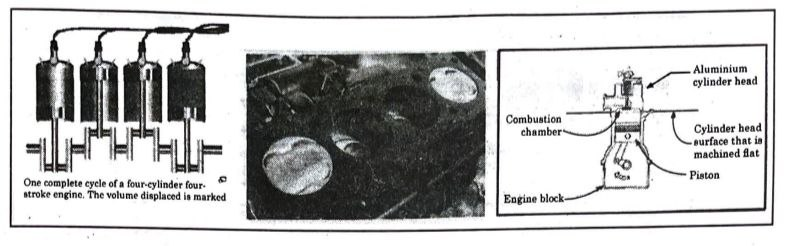
\includegraphics[width=1 \columnwidth]{engine.jpg}\\
			\caption{Engine}
			\label{fig:pic}  \end{figure}
		The cylinder bore in the form of circular cylinder open at the top is to be made from a metal sheet of area $ 75 \pi cm^2 $ \\
 	
		Based on the above information,answer the following questions:\\
		
			\begin{enumerate}
				\item if the radius of cylinder is r cm and height is h cm,then write the volme V of cylinder in terms of radius r.
					\\
				\item Find $ \frac{dV}{dr} $.
					\\
				\item \begin{enumerate}
						\item Find the radius of cylinder when its volume is maximum.\\
			
		\item For maximum volume,h>r.State true or false and justify.
				
			
				\end{enumerate}
			\end{enumerate}
\end{enumerate}
\end{document}
